% F2: the six steps from a 3DPW frame to an Anny label (Data 3.3). Only the tikzpicture; the chapter wraps it in a
% figure environment. Core TikZ only (no libraries). Steps: D part 3 "The six steps"; H 3.5 "How they are made";
% numbers from numbers_data.tex.
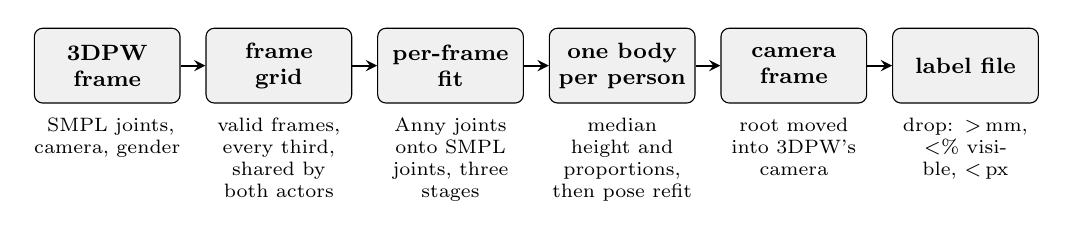
\begin{tikzpicture}[
    x=1cm, y=1cm, >=stealth,
    pstep/.style={draw, rounded corners=3pt, fill=black!6, minimum width=1.85cm, minimum height=0.95cm,
                 align=center, font=\footnotesize\bfseries, inner sep=2pt},
    note/.style={align=center, font=\scriptsize, text width=1.95cm, anchor=north, inner sep=1pt},
  ]
  \foreach \i/\name/\txt in {
      1/{3DPW\\frame}/{\DataSmplJoints{} SMPL joints, camera, gender},
      2/{frame\\grid}/{valid frames, every third, shared by both actors},
      3/{per-frame\\fit}/{Anny joints onto SMPL joints, three stages},
      4/{one body\\per person}/{median height and proportions, then pose refit},
      5/{camera\\frame}/{root moved into 3DPW's camera},
      6/{label file}/{drop: $>$\DataDropErr\,mm, $<$\DataDropVisPct\% visible, $<$\DataDropBox\,px}%
    }{
    \node[pstep] (s\i) at ({(\i-1)*2.18}, 0) {\name};
    \node[note] at ({(\i-1)*2.18}, -0.62) {\txt};
  }
  \foreach \a/\b in {1/2, 2/3, 3/4, 4/5, 5/6} {
    \draw[->, thick] (s\a.east) -- (s\b.west);
  }
\end{tikzpicture}
